\documentclass[10pt,twocolumn,letterpaper]{article}

\usepackage{cvpr}
\usepackage{times}
\usepackage{epsfig}
\usepackage{graphicx}
\usepackage{amsmath}
\usepackage{amssymb}

% Include other packages here, before hyperref.
\usepackage{color}
\newcommand{\high}[1]{\scriptsize{\text{\textcolor{red}{#1}}}}
\newcommand{\change}[1]{\textcolor{red}{#1}}

\usepackage{rotating}
% If you comment hyperref and then uncomment it, you should delete
% egpaper.aux before re-running latex.  (Or just hit 'q' on the first latex
% run, let it finish, and you should be clear).
\usepackage[pagebackref=true,breaklinks=false]{hyperref}
%\usepackage{multirow}

 \cvprfinalcopy % *** Uncomment this line for the final submission

\def\cvprPaperID{583} % *** Enter the CVPR Paper ID here
\def\httilde{\mbox{\tt\raisebox{-.5ex}{\symbol{126}}}}

% Pages are numbered in submission mode, and unnumbered in camera-ready
% \ifcvprfinal\pagestyle{empty}\fi
\begin{document}

%%%%%%%%% TITLE
\title{ The Synthesizability of Texture Examples}
\author{Dengxin Dai \quad Hayko Riemenschneider \quad Luc Van Gool\\
Computer Vision Lab, ETH Zurich, Switzerland\\
{\tt\small \{dai, hayko, vangool\}@vision.ee.ethz.ch}
% For a paper whose authors are all at the same institution,
% omit the following lines up until the closing ``}''.
% Additional authors and addresses can be added with ``\and'',
% just like the second author.
% To save space, use either the email address or home page, not both
}

\maketitle
%\thispagestyle{empty}

%%%%%%%%% ABSTRACT
\begin{abstract}
  
  Example-based texture synthesis~(ETS) has been widely used to
  generate high quality textures of desired sizes from a small
  example. However, not all textures are equally well reproducible
  that way. We predict how synthesizable a particular texture
  is by ETS. We introduce a dataset ($21,302$ textures) of
  which all images have been annotated in terms of their
  synthesizability.  We design a set of texture features, such as
  `textureness', homogeneity, repetitiveness, and irregularity, and
  train a predictor using these features on the data collection.  This
  work is the first attempt to quantify this image property, and we
  find that texture synthesizability can be learned and predicted. We
  use this insight to trim images to parts that are more synthesizable.  Also we suggest
  which texture synthesis method is best suited to synthesise a given
  texture. Our approach can be seen as `winner-uses-all': picking one
  method among several alternatives, ending up with an overall
  superior ETS method. Such strategy could also be considered for
  other vision tasks: rather than building an even stronger method,
  choose from existing methods based on some simple preprocessing.

\end{abstract}

%%%%%%%%% BODY TEXT

\section{Introduction}

\begin{figure} [!t]
  \centering
  \scalebox{0.93}{
   $ \begin{array}{cccc}
\hspace{-1.5mm}
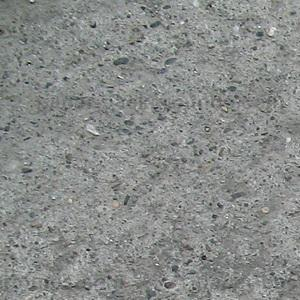
\includegraphics[width=0.33\linewidth]{./figs/fig1/google_concrete_441.jpg} & 
\hspace{-3mm}
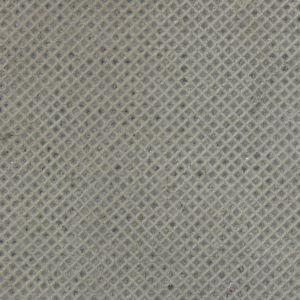
\includegraphics[width=0.33\linewidth]{./figs/fig1/google_concrete_476.jpg}&
\hspace{-3mm}
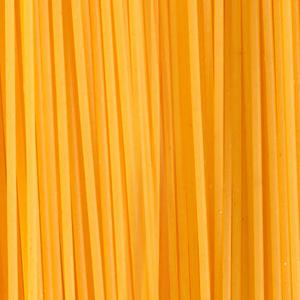
\includegraphics[width=0.33\linewidth]{./figs/fig1/bing2_food_19.jpg} \\
\scriptsize{\text{(a) \textcolor{red}{0.84}}} & \scriptsize{\text{(b) \textcolor{red}{0.80}}} & \scriptsize{\text{(c) \textcolor{red}{0.72}}} \\
% \hspace{-3mm}
% 455 0.56 feature.jpg 0.66   512 0.41   96 0.44 cliff3.jpg 0.40 
\hspace{-1.5mm}
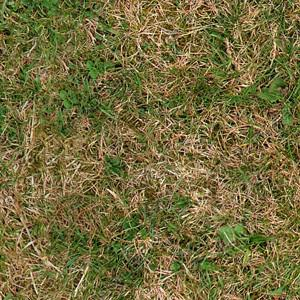
\includegraphics[width=0.33\linewidth]{./figs/fig1/google_grass_566.jpg} & 
\hspace{-3mm}
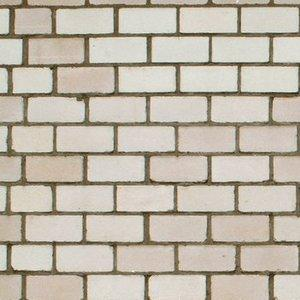
\includegraphics[width=0.33\linewidth]{./figs/fig1/google_brick_190.jpg}&
\hspace{-3mm}
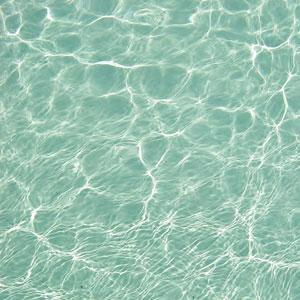
\includegraphics[width=0.33\linewidth]{./figs/fig1/google_water_703.jpg} \\
\scriptsize{\text{(d) \textcolor{red}{0.57}}} & \scriptsize{\text{(e) \textcolor{red}{0.54}}} & \scriptsize{\text{(f) \textcolor{red}{0.51}}} \\
\hspace{-1.5mm}
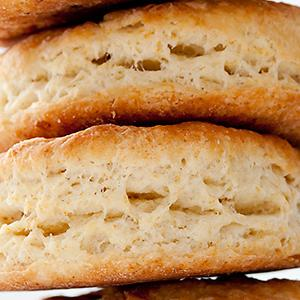
\includegraphics[width=0.33\linewidth]{./figs/fig1/flickr_biscuit_194.jpg} & 
\hspace{-3mm}
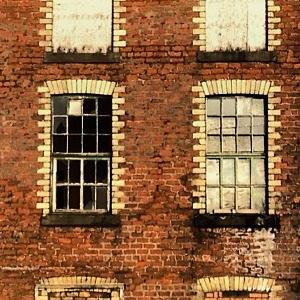
\includegraphics[width=0.33\linewidth]{./figs/fig1/flickr_brick_233.jpg}&
\hspace{-3mm}
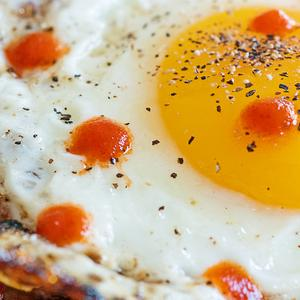
\includegraphics[width=0.33\linewidth]{./figs/fig1/flickr_chips_144.jpg} \\
\scriptsize{\text{(g) \textcolor{blue}{0.41}}} & \scriptsize{\text{(h) \textcolor{blue}{0.35}}} & \scriptsize{\text{(i) \textcolor{blue}{0.32}}} \\
\hspace{-1.5mm}
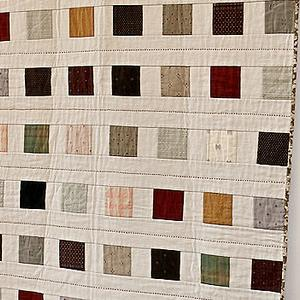
\includegraphics[width=0.33\linewidth]{./figs/fig1/flickr_Fabric_471.jpg} & 
\hspace{-3mm}
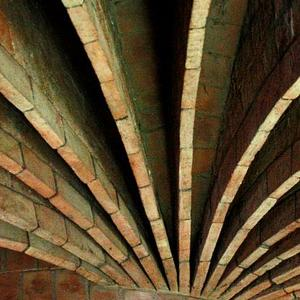
\includegraphics[width=0.33\linewidth, height=27.5mm]{./figs/fig1/flickr_brick_215.jpg}&
\hspace{-3mm}
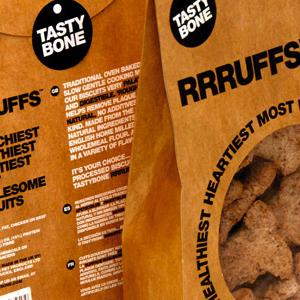
\includegraphics[width=0.33\linewidth]{./figs/fig1/bing2_food_75.jpg} \\
\scriptsize{\text{(j) \textcolor{blue}{0.28}}} & \scriptsize{\text{(k) \textcolor{blue}{0.18}}} & \scriptsize{\text{(l) \textcolor{blue}{0.14}}} \\
% \hspace{-3mm}
% 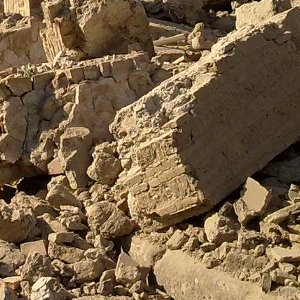
\includegraphics[width=0.25\linewidth]{./figs/fig1/wall.jpg} \\
\end{array}$}
\caption{Synthesizability of texture examples detected by
  our system. The values are in $[0, 1]$ and a higher value means the example is easier
 to synthesize. All images are of $300\times 300$ pixels.}
  \label{fig:synlity}
\end{figure}


%% ABILITY TO MEASURE synthesizability
A substantial amount of work has been devoted to synthesising textures
from examples~\cite{Heeger:95,
  Portilla:2000:IJCV,Efros:sig2001,Kwatra:2003, Lefebvre:2005:sig,
  Ma:2011,dai:facade:iccv13}. We will refer to such example-based
texture synthesis as `ETS' in the remainder of this paper. Even if the
set of textures that can be successfully synthesised that way has
steadily been growing, it is often not clear beforehand whether ETS
would be successful for a specific texture sample. It would be
interesting if we were able to predict its synthesizability -- how
well its underlying visual patterns can be re-synthesized by learning
only from the sample. Even if challenging, the task may be doable,
given that other qualitative image characteristics could be
quantified, like quality~\cite{image:quality},
memorability~\cite{image:memorability}, or
interestingness~\cite{image:interestingness}.


%% PROBLEM WITH TEXTURES IN THE WILD
While ETS has proven to be a powerful tool to generate large-scale
textures~\cite{WLKT09}, providing texture examples is not
straightforward~\cite{lockerman2013arxiv}. ETS systems typically
expect a rectangular sample image, representing a head-on view of a
flat, outlier-free textured surface. Not just any example image
returned by an image searching engine (by typing keywords) will do.
Such retrieved images usually contain outliers, cluttered backgrounds,
distorted texture surfaces, or even objects and complex scenes. Being
able to rank retrieved images in terms of their synthesizability can
then at least perform an initial selection. It can also be used to
trim images to regions with good synthesizability, by e.g.~removing
undesirable background. Furthermore, synthesizability can help select
an appropriate ETS method. The optimal approach -- also taking into
account speed and stability -- will depend on the texture and the
application. Quilting~\cite{Efros:sig2001} is very potent, for
instance, but will tend to produce verbatim repetitions that become
salient when larger areas need to be synthesized. It would be good if
in such case one could take recourse to an alternative method that
does not produce such issues. Last but not least, studying
synthesizability as a general image property is interesting {\em per
  se}.

Fig.~\ref{fig:synlity} shows the synthesizability scores assigned to some texture samples 
by our system. Fig.~\ref{fig:roi} illustrates the trimming of an image to its most
synthesizable, rectangular regions (the red cut-outs).

In order to learn image synthesizability and evaluate its performance, we have collected
a fairly large texture dataset of $21,302$ texture images. This dataset has been manually annotated 
in terms of the synthesizability of each image. The synthesizability is characterised as the 
`goodness' of the `best' synthesis result as obtained by a set of ETS methods. The `goodness' is quantified 
as one of three levels: good, acceptable, and bad. See Fig.~\ref{fig:dataset} for examples. 

% {\bf IT IS NOT CLEAR WHAT KIND OF ANNOTATIONS
% THESE ARE: MANUALLY DONE… OR THE SCORES AUTOMATICALLY GIVEN BY OUR METHOD? IF MANUALLY
% DONE, IT IS NOT CLEAR HOW TO COME UP WITH NUMBERS AS IN FIG.1, SO FAR THE GOOD-ACCEPTABLE-BAD 

% CLASSIFICATION HAS NOT BEEN INTRODUCED.}

As to the automated synthesizability scoring, a series of features
that would seem to be connected with the task are defined.  A scoring
function is then learned from the collection of annotated data.  The
experimental results show that automated synthesizability scoring is
possible.

Our main contribution are: (1) to learn the image property
synthesizability methodologically; (2) to design several novel
features for qualitative texture analysis (esp. `textureness',
homogeneity, repetitiveness, and irregularity); and (3) to offer a fairly
large texture dataset together with synthesizability annotations;


The remainder of the paper is organized as follows.
Sec.~\ref{sec:related} reports related work.
Sec.~\ref{sec:data} is devoted to our dataset, followed by our features and learning method in Sec.~\ref{sec:feature}.
Sec.~\ref{sec:experiment} presents our experiments and Sec.~\ref{sec:conclusion} concludes. 


\section{Related work}
\label{sec:related}

\textbf{Example-based texture synthesis.}  Techniques of example-based
texture synthesis can be broadly categorized into four categories:
feature-oriented synthesis~\cite{Heeger:95, Debonet:97,
  Portilla:2000:IJCV, random:phase}, Markov Random Fields (MRFs)
methods~\cite{paget:tip98, zhu:frame, Zalesny05}, neighborhood-based
methods~\cite{Efros:sig2001, Kwatra:2003, Kwatra:tog:2005,
  dai:facade:iccv13}, and tile-based methods~\cite{Cohen:2003:wang,
  Liu:2004:NTA}.  The first group learns the statistics of carefully
designed features and leads the synthetic images to have/achieve
similar values, e.g. color histograms~\cite{Heeger:95}, multi-band
spatial frequencies~\cite{Debonet:97}, and wavelet
features~\cite{Portilla:2000:IJCV}. This group of methods are stable
and do not generate verbatim repetition, but the main challenge lies
in designing a common set of features that is able to capture the
essence of all kinds of textures.  The second group considers textures
as instances of MRFs. Parameters of the MRFs are estimated from the
texture examples and new textures are then sampled from the
model. Multi-scale neighborhood-based MRFs are learned
in~\cite{paget:tip98} and pairwise clique-based MRFs
in~\cite{Zalesny05}. This strand is theoretically well-founded, but is
computationally expensive. The third group generate textures by
copying pixels or patches from the exemplar inputs~\cite{Efros:1999,
  Efros:sig2001, Kwatra:2003, Kwatra:tog:2005,
  dai:facade:iccv13}. Unlike the first two groups they do not provide
cues for texture analysis, but are often more efficient and tend to
work for a larger variety of textures. The last group assemble new
textures out of a set of (rectangular) tiles cropped from example
images. This stream of methods are very efficient once the tiles are
estimated. However, identifying these tiles is non-trivial:
\cite{liu:ijcv:05} handled this problem by estimating the translation
symmetries and \cite{dai:facade:iccv13} through semantic labeling.

\textbf{Texture recognition.}  Our work is also related -- albeit
rather weakly -- to material recognition. Features for material
classification include statistics of filter
responses~\cite{texton:2001, Manjunath96, Schmid01}, joint intensity
distributions within a compact neighborhood ~\cite{material:pami:09,
  sorted:texture}, geometric features over topographic
maps~\cite{xia:texture}, and high-level semantic
attributes~\cite{semantic:texture}.  Similarly, we need
to design appropriate features for this new task.


%%%%%%%%%%%%%%%%%%%%%%%%%%%%%%%%%%%%%%%%%%%%%%%%%%%%%%%%%%%%%%%%%%%%%%%%%%

\section{Data collection}
\label{sec:data}
Although it stands to reason that some textures are easier to
synthesise than others, quantifying this expectation has not been
addressed. In order to learn to predict synthesizability, we collected
a texture dataset and annotated it in terms of
synthesizability. $40,000$ images were downloaded from Google, Bing,
and Flickr by providing $60$ keywords. The keywords used are to cover
common material classes such as glass, water, stone, plastic, fabric,
leather, metal and paper, and to cover common geometric texture
attributes such as stochastic, repetitive, lined, speckled, wrinkled
and cracked. All images were truncated to $300 \times 300$ pixels,
with images smaller than this not being used. Since the retrieved
images are very `noisy', with some not showing textures, being of low
quality, or being severely watermarked, we made a manual selection for
the truncated images. Finally, we ended up with a dataset of $21,302$
texture samples.

For the annotation, we characterize the synthesizability of a texture
as the `goodness' of the best synthesized image among those generated
by a selected set of ETS methods. A good synthesized image should be
as similar as possible to the input example and should not have
visible artifacts such as seams, blocks and ill-shaped edges, and
should not contain salient repetitions of sub-patterns in a verbatim
fashion, if that is not the case in the original. Since no single ETS
method performs better than all others on all kinds of textures, the
annotator got the choice between the results of four specific methods,
that are based on different methodologies: an image quilting
method~\cite{Efros:sig2001}, a multi-scale Markov Random Field (MMRF)
method~\cite{Zalesny05}, a wavelet-based parametric
method~\cite{Portilla:2000:IJCV}, and a random phase
synthesis~\cite{random:phase}. While future work will probably yield
more powerful ETS methods still, this dataset constitutes an initial
benchmark, based on the current state-of-the-art in ETS. The final
outcome of the annotation for a texture example is the `goodness' of
the synthesized result (among the 4) that an expert annotator
considered best. This goodness was expressed as one of 3 levels: good,
acceptable, and bad, assigned synthesizability scores of $1$, $0.5$
and $0$, resp. The `best' method of each texture example was also
recorded to learn which method is the best to synthesize a given
texture example. This was only performed for `good' and `acceptable'
images; `bad' ones were assigned to `NULL'.  Fig.~\ref{fig:dataset}
shows examples of such annotation. In total, $25.5\%$ samples were
labeled bad, $39.7\%$ acceptable and $34.8\%$ good.

%The dataset (incl. images and synthesizability
%scores) is publicly available at the project page.

\begin{figure} [!t]
  \centering
   $ \begin{array}{cccc}
\hspace{-1.5mm}
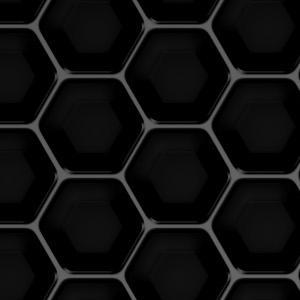
\includegraphics[width=0.23\linewidth]{./figs/dataset/87.jpg} & 
\hspace{-3mm}
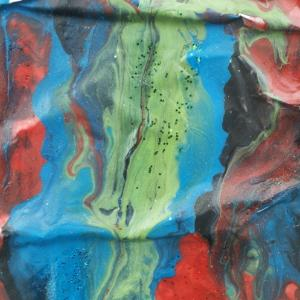
\includegraphics[width=0.23\linewidth]{./figs/dataset/flickr_cardboard_211.jpg} & 
\hspace{-3mm}
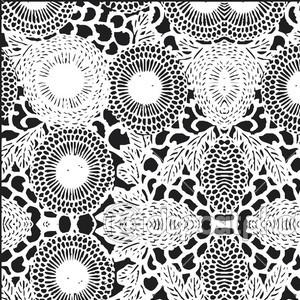
\includegraphics[width=0.23\linewidth]{./figs/dataset/google_flower_169.jpg} \\ 
\hspace{-1.5mm}

\includegraphics[width=0.32\linewidth]{./figs/dataset/87syn.jpg} & 
\hspace{-3mm}
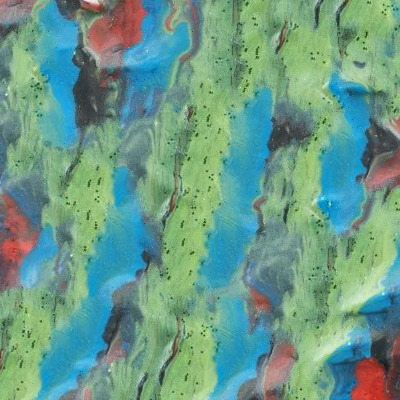
\includegraphics[width=0.32\linewidth]{./figs/dataset/flickr_cardboard_211_m.jpg} & 
\hspace{-3mm}
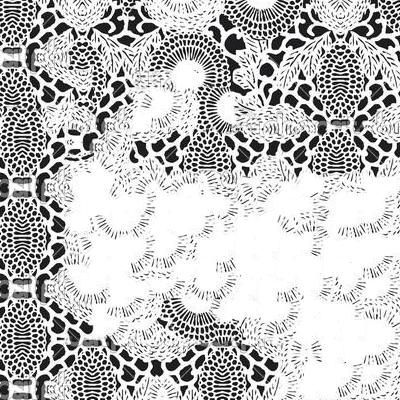
\includegraphics[width=0.32\linewidth]{./figs/dataset/google_flower_169_q.jpg} \\ 

% \hspace{-1.5mm}
% 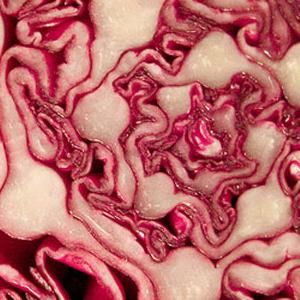
\includegraphics[width=0.23\linewidth]{./figs/dataset/bing2_food_113.jpg} & 
% \hspace{-3mm}
% 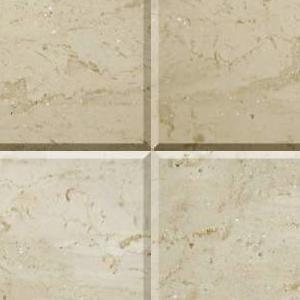
\includegraphics[width=0.23\linewidth]{./figs/dataset/bing2_floor_118.jpg} & 
% \hspace{-3mm}
% 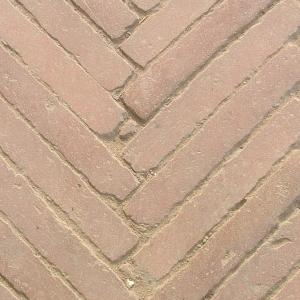
\includegraphics[width=0.23\linewidth]{./figs/dataset/bing2_floor_41.jpg} \\ 
% \hspace{-1.5mm}
% 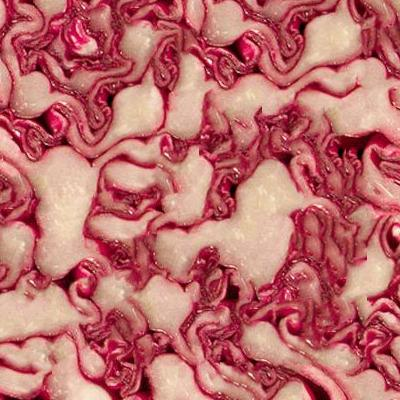
\includegraphics[width=0.33\linewidth]{./figs/dataset/bing2_food_113_q.jpg} & 
% \hspace{-3mm}
% 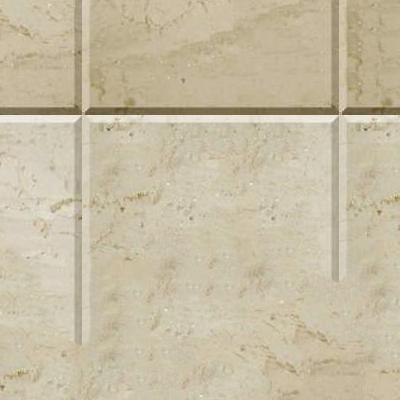
\includegraphics[width=0.33\linewidth]{./figs/dataset/bing2_floor_118_q.jpg} & 
% \hspace{-3mm}
% 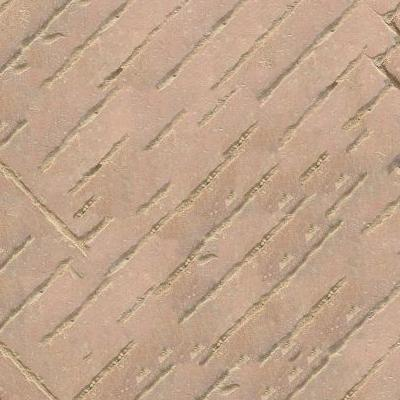
\includegraphics[width=0.33\linewidth]{./figs/dataset/bing2_floor_41_q.jpg} \\ 

\hspace{-1.5mm}
\scriptsize{\text{(a) good, Quilting}} & 
\hspace{-3mm}
\scriptsize{\text{(b) acceptable, MMRF}} & 
\hspace{-3mm}
\scriptsize{\text{(c) bad, NULL}}  \\

\end{array}$
\caption{Three texture examples from our dataset with their
  annotations of synthesizability. Top: texture exemplars;
  bottom: synthesized textures. }
  \label{fig:dataset}
\end{figure}


%%%%%%%%%%%%%%%%%%%%%%%%%%%%%%%%%%%%%%%%%%%%%%%%%%%%%%%%%%%%%%%%%%%%%%%%%

\section{Learning image synthesizability} 
\label{sec:feature}
In this section, we investigate the visual features relevant to 
image synthesizability. We start from general image features, to move
on to our designed texture features, and to the learning method.

%=======================================================================

\subsection{General features}

% \textbf{Wavelets}. Wavelets have been widely used for texture
% analysis, so we allowed them to contribute to image synthesizability. 
% The complex pyramid wavelet transform on $4$ pyramid levels, with 
% sp3Filters, was used, due to its promising performance on texture 
% analysis/synthesis~\cite{Portilla:2000:IJCV}.


\textbf{Local patterns}. Local binary patterns (LBP)~\cite{lbp:2002}
have been widely used in texture recognition and such features 
achieved s-o-a classification performance~\cite{sorted:texture}. Thus, 
we included uniform LBP.

\textbf{Filter responses}. Using image filters has become one of the
most popular tools for texture analysis~\cite{texton:2001, Manjunath96}
and synthesis~\cite{zhu:frame}. Thus, filter bank responses may 
be helpful for learning synthesizability too. The Schmid Filter
Bank~\cite{Schmid01} is employed with 13 rotationally invariant
filters at $5$ scales. 

\textbf{GIST features}. Frequency analysis has proven very useful for
texture analysis/synthesis~\cite{vangool83, Manjunath96, Debonet:97}, so features 
of this kind can best be included here as well. GIST~\cite{gist} is used, 
where the implementation resizes images to $256 \times 256$ pixels, only
considers one grid, and produces a feature vector of dimension $20$.

% \textbf{Self-similarity}. Sufficiently small patches of textures are 
% self-similar in appearance. Thus, it is interesting to evaluate the 
% self-similarity feature~\cite{self:similarity}. We averaged the 
% self-similarity
% vectors of all pixels in an image to represent its self-similarity.

% \textbf{Complexity}. We follow~\cite{image:interestingness} to measure
% the complexity of an image by comparing its JPEG compressed size
% against its uncompressed size. The lower the compression rate, the 
% more complex the texture pattern is. This measure is interesting as
% JPEG has been conceived with human image perception in mind. 

% \textbf{Colorfulness}. The complexity of a texture is also reflected 
% by its colorfulness: the more colors are
% involved in the texture patterns, the more complex the textures tend
% to be. We measure colorfulness as proposed by Datta and Wang~\cite{aesthetic:eccv06}, \ie
% the Earth Mover distance of the color histogram of the texture image
% to a uniform color histogram (representing the most colorful image).
% The smaller the distance, the more colorful (complex) the texture.

% \textbf{Edge length}. It is observed that examples with long edges are
% harder to synthesize than those with shorter edges. A histogram of the
% length of edges is used to characterize this property. We use the
% Canny edge detector~\cite{canny:edge} for edge detection, with the
% high and low thresholds put to $0.6$ and $0.24$, resp.  The histogram
% of $8$ bins is used with the following separating positions: $2, 5,
% 10, 20, 50, 100, 200$.


% SHAPE PRIMITIVES
% \textbf{Shape primitives}.  Apart from generic edges, we further
% investigate the presence of basic shape primitives.  Straight lines
% and corners may be easier to reproduce than complex, irregular shapes.
% For this purpose, we extract local edge fragments with the Canny
% edges.  These local fragments are described by a `self-embedded local
% shape descriptor'~\cite{hayko:eccv2010} which captures the local shape
% by dense angular representation.  We train a vocabulary of shape
% fragments by clustering on the Brodatz texture datasets.  A histogram
% over these shape fragments is then used to describe the presence of
% local shape primitives.


% \textbf{Entropy}.  To capture the complexity of an image, image
% entropy is also measured. Entropy is a statistical measure of
% randomness that can be used to characterize the texture of the input
% image.

% \textbf{structures} cf.~\cite{tsmoothing2012}: texture and main
% structure exhibit completely different properties, makign them
% surprisingly decomposable. We do not assume specific regularity and
% symmetry of the texture patterns: non-uniform and anistropic texture,
% can be handled in a unified framework.
% We do not assume or manually determine the type of textures, as the
% patterns could vary a lot in different examples. 

% Relative Total Variation (RTV) is simple and yet very effective to
% make main structures stand out, thanks to the characteristics of $D$
% and $\phi$.

% \textbf{Patch PCA}.  The randomness of a texture is signaled by the
% intrinsic dimensionality of local texture patches.
% Patches from random textures normally have a higher intrinsic
% dimensionality than patches from smooth textures. Therefore, we
% perform principal component analysis on local patches sampled from the
% texture image and use their intrinsic dimensionality as a feature.
% Specifically, we sampled patches of $20\times 20$ pixels, centered at
% every pixels of the image, and searched for the dimensionality that
% keeps $85\%$ of the energy. This intrinsic dimensionality normalized 
% by the original dimensionality of the patches, i.e. $400$, is used. 

%This feature has been used
%already for image quality prediction~\cite{blind:quality:cvpr11}.

% Textureness

\subsection{Designed features}

\begin{figure} [!t]
  \centering
\scalebox{0.94}{
   $ \begin{array}{cccc}
\hspace{-1.5mm}
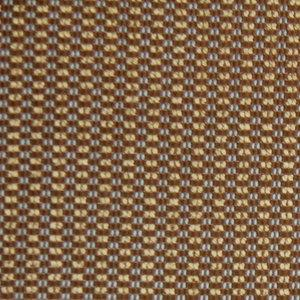
\includegraphics[width=0.33\linewidth]{./figs/repet/1.jpg} & 
\hspace{-3mm}
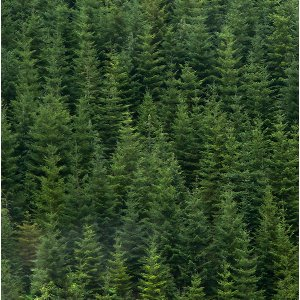
\includegraphics[width=0.33\linewidth]{./figs/repet/forest.jpg} & 
\hspace{-3mm}
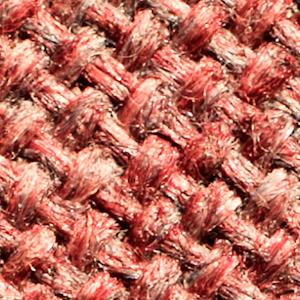
\includegraphics[width=0.33\linewidth]{./figs/repet/273.jpg} \\ 
\scriptsize{\text{(a) 8.82}} & \scriptsize{\text{(b) 3.84}} & \scriptsize{\text{(c) 3.73}}  \\
\hspace{-1.5mm}
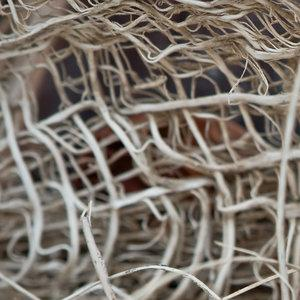
\includegraphics[width=0.33\linewidth]{./figs/repet/439.jpg} & 
\hspace{-3mm}
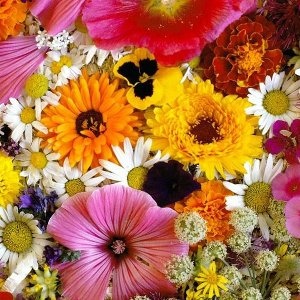
\includegraphics[width=0.33\linewidth]{./figs/repet/flower2.jpg} & 
\hspace{-3mm}
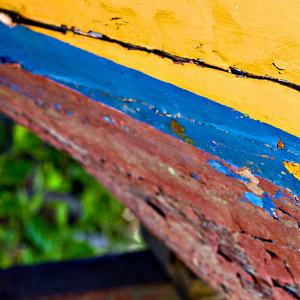
\includegraphics[width=0.33\linewidth]{./figs/repet/832.jpg} \\ 
\scriptsize{\text{(d) 3.12}} & 
\scriptsize{\text{(e) 1.80}} & 
\scriptsize{\text{(f) 1.63}}  \\

\end{array}$}
\caption{The homogeneity of texture examples detected by our
  method. Images are all of $300 \times 300$ pixels.}
  \label{fig:homo}
\end{figure}

% \textbf{Edge coverage}.  
% \textbf{Attributes} lined or circled~\cite{semantic:texture}? 

\textbf{`Textureness'}. Objects and scenes are more difficult to
synthesize than actual textures. We train a classifier to distinguish
textures from objects and scenes. The UIUC texture
dataset~\cite{UIUC:Texture} delivered the positive samples (textures),
and the 15-Scene dataset~\cite{lazebnik:cvpr06} the negative ones
(objects/scenes). Linear SVMs were used as the classifier with
GIST~\cite{gist} as the feature. The classification score is taken as
`textureness'.

% Homogeneity
\textbf{Homogeneity}. Homogeneous textures are easier to synthesize
than heterogeneous ones. Thus, it is desirable to have a feature
measuring homogeneity. One possibility is based on co-occurrence
matrices~\cite{texture:analysis}, but is low-level and quite noise
sensitive. We here propose a simple, yet more robust method based on
our definition of homogeneity.

\noindent 
\textbf{Definition:} The homogeneity of an image is the expectation of
visual similarity between two randomly-chosen local regions of the image.

In particular, given an image $X \in \mathbb{R}^{H\times W}$, we
measure the average similarity over $T$ ($80$ in the implementation)
trials.  In trial $t$, two regions $R_1^t$ and $R_2^t$ are sampled
from $X$, and their distance $d(R_1^t, R_2^t)$ is measured. The
homogeneity of $X$ is then:
\begin{equation}
  \label{eq:repet}
\text{Hom}(X) = \frac{1}{T}\sum_{t=1}^T \frac{1}{d(R_1^t, R_2^t)}.  
\end{equation}
where $d(\cdot, \cdot)$ is the Euclidean distance, $R_1^t$ and $R_2^t$
are of the same size $\lfloor H/3 \rfloor \times \lfloor W/3 \rfloor$,
and the positions of their top-left corners are sampled uniformly, at
random from $\{(i,j): i\in\{1, ..., \lfloor 2H/3 \rfloor \}, j\in \{1,
..., \lfloor 2W/3 \rfloor \} \}$.  The regions are represented with
bag-of-words. The dictionary is learned from $X$ by k-means with $30$
`word' centres and with $10\times 10$ patches around every pixel (RGB
values are used). See Fig.~\ref{fig:homo} for the homogeneity of six
texture examples detected by the method.  Our homogeneity is more
effective than the co-occurrence one ~\cite{texture:analysis} because
it uses regions rather than single pixels. It is also more robust
because the word histograms yield some spatial invariance. 
 
%  \textbf{low-rank texture} 
% Our intuitive distinction between these two kinds
% of data is that textur
% ~\cite{low:rank:texture:ijcv12}. 

\begin{figure} [!t]
  \centering \scalebox{0.94}{
   $ \begin{array}{cccc}
\hspace{-1.5mm}
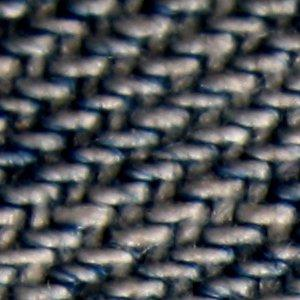
\includegraphics[width=0.33\linewidth]{./figs/repetitiveness/60.jpg} & 
\hspace{-3mm} 
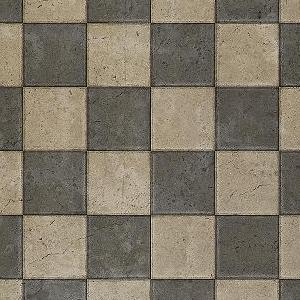
\includegraphics[width=0.33\linewidth]{./figs/repetitiveness/bing2_floor_201.jpg} & 
\hspace{-3mm}
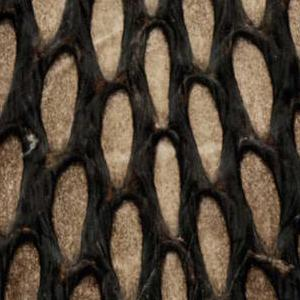
\includegraphics[width=0.33\linewidth]{./figs/repetitiveness/bing2_animal_19.jpg} \\ 
\scriptsize{\text{(a) 76.4}} &
 \scriptsize{\text{(b) 70.5}} & 
\scriptsize{\text{(c) 66.5}}  \\
\hspace{-1.5mm}
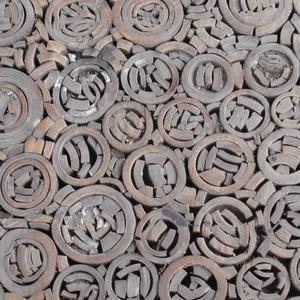
\includegraphics[width=0.33\linewidth]{./figs/repetitiveness/bing2_floor_78.jpg} & 
\hspace{-3mm}
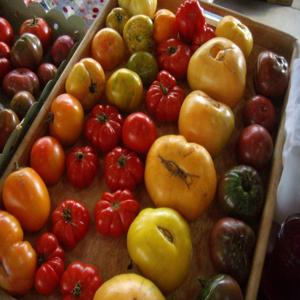
\includegraphics[width=0.33\linewidth]{./figs/repetitiveness/10rep.jpg} & 
\hspace{-3mm}
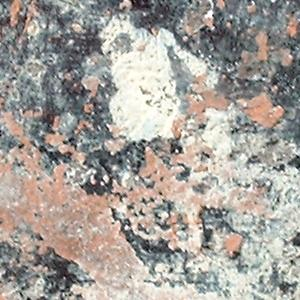
\includegraphics[width=0.33\linewidth]{./figs/repetitiveness/bing2_floor_24.jpg} \\ 
\scriptsize{\text{(d) 49.7}} & 
\scriptsize{\text{(e) 39.4}} & 
\scriptsize{\text{(f) 32.4}}  \\
% \hspace{-1.5mm}
% \includegraphics[width=0.33\linewidth]{./figs/repetitiveness/cv/cv_60.jpg} & 
% \hspace{-3mm}
% \includegraphics[width=0.33\linewidth]{./figs/repetitiveness/cv/cv_2.jpg} & 
% \hspace{-3mm}
% \includegraphics[width=0.33\linewidth]{./figs/repetitiveness/cv/cv_9rep.jpg} \\ 
% \scriptsize{\text{(g): NCC map of (a)}} & 
% \scriptsize{\text{(h): NCC map of (d)}} & 
% \scriptsize{\text{(i): NCC map of (f)}}  \\
\end{array}$}
\caption{The repetitiveness of texture examples detected by our
  method. Images are all of $300 \times 300$ pixels.
% : (a)-(f). 
% (g), (h), and (i) show the NCC results of (a), (d),
%   and (f) resp., where the red rectangles indicate region $R$'s.
}
  \label{fig:repet}
\end{figure}

% Repetitiveness
\textbf{Repetitiveness}. Textures are usually referred to as visual
surfaces composed of repeating patterns, that are similar in
appearance~\cite{WLKT09}. FFT features, of which the power spectrum is
directly related to auto-correlation, have been used very early
on~\cite{vangool83, texture:analysis, liu:texture:96}. For periodic patterns, the
auto-correlation function is strongly peaked. Here we propose a
related measure, also aimed at capturing imperfect repetitions 
(Fig.\ref{fig:repet}), that is defined in the spatial domain.

The method draws on normalized cross correlation (NCC): an image $X
\in \mathbb{R}^{H\times W}$ is cross-correlated with itself,
generating an NCC matrix $D\in \mathbb{R}^{(2H-1)\times (2W-1)}$. The
elements in the matrix are divided by the number of pixels involved in
their calculation (different overlap as the image is shifted across
itself). The borders of the matrix are not used due to the insufficient
overlap there. The idea is that  if $X$ is repetitive, the following two
properties should hold: (1) for a random moderate-sized region $R$ of
$D$, the difference between its maximum value and its minimum value
should be large; (2) the minimum values of a set of randomly sampled
$R$'s (of the same size) should be very close.  The philosophy behind
(1) is that for repetitive textures, the auto-correlation function
should exhibit peaks and valleys. Property (2) is derived from the fact
that the distances between all `repeated' versions should be
similar.

Denoting by $Max(R_t)$ and $Min(R_t)$ the maximum and minimum values
of the $t$th region $R_t$, we quantify the repetitiveness of $X$ as
\begin{equation} 
\text{Rep}(X) = \left( \frac{1}{T} \sum_{t=1}^T \frac{Max(R_t)}{Min(R_t)} \right)
                \times \frac{1}{\sigma(Min(R_t))}
\end{equation}
where $T$ ($80$ in the implementation) is the number of randomly
sampled $R$'s in $D$, and $\sigma(z)$ is the standard deviation of
$z$. The size of $R$ is set to $\lfloor H/5 \rfloor \times \lfloor W/5
\rfloor$. Too small a size cannot capture large-scale repetition, and
too large a size looses discrimination power.  See
Fig.~\ref{fig:repet} for examples of detected
repetitiveness. Repetitiveness is akin to the Harmonicity feature
of~\cite{liu:texture:96}, but repetitiveness is more robust due to its
pooling over local regions.

\textbf{Irregularity}. Irregular textures are harder to synthesize
than regular ones~\cite{Liu:2004:NTA}, so we conjecture that the
irregularity of textures is also relevant to their
synthesizability. Although the irregularity of textures has been
suggested before, we still lack a method to measure it
computationally. We propose Ensemble Composition (EC) for such
quantification. The idea is that if a texture is regular, composing
any of its regions using image chunks from outside will be
\emph{cheap} (See images in Fig.~\ref{fig:irreg} to get the idea).  We
again do this over an ensemble -- over $T$ trials ($80$ in the
implementation), we use the average composition energy to indicate
texture irregularity. In the $t$-th trial, given an image $X$, we
denote by $R^t$ the region to compose, and by $Y^t$ the rest of the
image. The composition should have two properties: (1) the composited
region should be similar to $R^t$; (2) the chunks from $Y^t$ should be
as continuous (large) as possible.

We formulate the composition task
as a graph labeling problem with the following energy: 
%  with the spatial offsets between composed
% pixels and composing pixels as labels, and pixel values of $R^t$ as observed data. The formulation is:
\begin{equation}
  \label{eq:regu:energy}
  E(R^t) = \sum_{i\in R^t}D_i(l_i) + \lambda \sum_{\{i,j\} \in \mathcal{N}}V(l_i, l_j)
\end{equation}
where $l_i$ is the label assigned to pixel $i$ in region $R^t$, and
$\mathcal{N}$ is the neighborhood set of pixels in $R^t$. The label
$l_i$ represents the pre-defined offsets $\bold{s}_{l_i}$ between the
composed pixels and composing pixels in the 2D image domain, that is,
$l_i \in \{1, ..., \#(X)\}$.  $D_i(l_i)$ denotes the cost of assigning
the $l_i$th label to the $i$th pixel of $R^t$, and it is defined to
reflect the similarity of pixel $i$ and corresponding shifted pixel
$i+\bold{s}_{l_i}$. To counteract noise, we use the Euclidean distance
between the Schmid Filter responses~\cite{Schmid01}; positive infinity
is used when the shifted position falls outside of $Y^t$. For the
smoothing term $V(l_i, l_j)$, we use the Potts model, i.e. $V(l_i,l_j)
= 0$ if $l_i = l_j$ and $1$ otherwise. $\lambda$ is set to $50$ to
balance the two energy terms.  By performing $T$ trials, the
irregularity of texture $X$ is then defined as:
\begin{equation}
  \label{eq:regularity}
  \text{IReg}(X) = \frac{1}{T} \sum_{t=1}^{T}E(R^t). 
\end{equation}
The energy is optimized by multi-label graph-cuts~\cite{graphcut}.  In
order to speed the optimization up, we employed the technique of
dominant offsets proposed in~\cite{He:completion:eccv12} -- only the
dominant offsets ($60$ in our implementation) were considered as the
labels. We also approximated the nearest neighbor search (for
dominant offsets) by clustering patches into clusters ($200$ in our
case) -- patches in the same cluster are considered as neighbors. Our
texture irregularity is similar to Boiman's image
irregularity~\cite{Boiman:07}, but we focus on textures and
compose the image from itself instead of composing general scenes from a
dataset. Also, we provide an irregularity score for a given image by a
new ensemble method.

\begin{figure} 
  \centering \scalebox{0.94}{
   $ \begin{array}{cccc}
\hspace{-1.5mm}
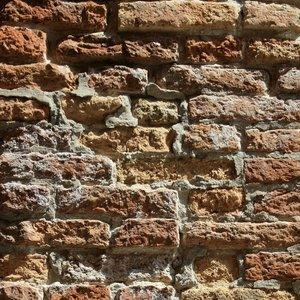
\includegraphics[width=0.33\linewidth]{./figs/regularity/403.jpg} & 
\hspace{-3mm} 
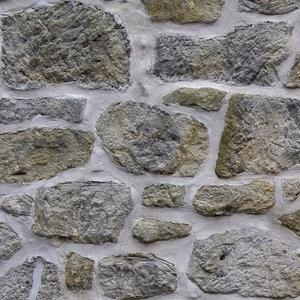
\includegraphics[width=0.33\linewidth]{./figs/regularity/13.jpg} & 
\hspace{-3mm}
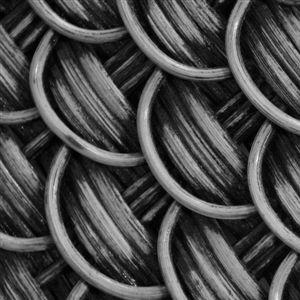
\includegraphics[width=0.33\linewidth]{./figs/regularity/90.jpg} \\ 
\scriptsize{\text{(a) 0.22}} & \scriptsize{\text{(b) 0.14}} & \scriptsize{\text{(c) 0.12}}  \\
\hspace{-1.5mm}
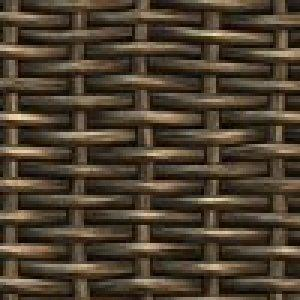
\includegraphics[width=0.33\linewidth]{./figs/regularity/57.jpg} & 
\hspace{-3mm}
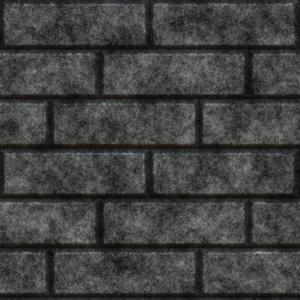
\includegraphics[width=0.33\linewidth]{./figs/regularity/28.jpg} & 
\hspace{-3mm}

\includegraphics[width=0.33\linewidth]{./figs/regularity/google_Paper_100.jpg} \\ 
\scriptsize{\text{(d) 0.10}} & 
\scriptsize{\text{(e) 0.08}} & 
\scriptsize{\text{(f) 0.05}}  \\
\end{array}$}
\caption{The irregularity of texture examples captured by Ensemble
  Composition. Images are all of $300 \times 300$ pixels.}
  \label{fig:irreg}
\end{figure}

It is noteworthy that homogeneity, repetitiveness, and regularity
capture different properties. For instance, the texture in
Fig.~\ref{fig:homo}(b) is homogeneous, but not repetitive and not
regular. The texture in Fig.~\ref{fig:irreg}(f) is homogeneous and
regular, but not repetitive.  In a nutshell, the 4 designed features
are not orthogonal (\eg repetitive textures are normally regular as
well), but are complementary nonetheless. Moreover, we do not claim
that the $7$ features (general + designed) are optimal or
exhaustive. Other features such as entropy, coarseness,
directionality, could also be relevant to synthesizability.

\subsection{Learning method}
We attempt to computationally quantify texture synthesizability and to
use this to aid synthesis. To those ends, we train (1) a regression
model on the synthesizability scores ($1$, $0.5$ and $0$) to predict
the synthesizability of a given image, and (2) an additional
classifier to suggest the `best' ETS method to synthesize it.  Random
Forest~\cite{randomforest} was used for both training tasks due to its
fast speed. $30$ trees were used for the forest.

%%%%%%%%%%%%%%%%%%%%%%%%%%%%%%%%%%%%%%%%%%%%%%%%%%%%%%%%%%%%%%%%%%

\section{Experiments}
\label{sec:experiment}
% In this section, we evaluate the task of learning synthesizability,
% and its usefulness for trimming texture examples and recognizing
% texture classes.

\subsection{Learning synthesizability}

In this section, we evaluate the contribution of all features to the
prediction of synthesizability and to what degree it is learnable.
All $7$ single features and their $3$ combinations were
evaluated. The $3$ combinations are: combination of the $3$
general features (General), combination of the $4$ designed features
(Designed), and combination of all features (All).  $30\%$ of the
dataset images were used for training, the rest for testing. We report
results over $5$ random training-testing splits. For evaluation, we
performed two retrieval tasks and evaluated the average precision for
different levels of recall: (1) retrieve images with `good' scores
($>=$good); (2) retrieve images with `good' or `acceptable' scores
($>=$acceptable).


\textbf{Quantitative evaluation}. Table~\ref{table:contribution} shows
the results for different, single as well as combined features when 
recall is set to $1$, and Fig.~\ref{fig:curve} shows the results for 
different levels of recall when all features are used. The table shows 
that every single feature is helpful. Homogeneity performs the best. 
It is also interesting that the combination of the 4 designed features 
performs substantially better than the combination of the 3 general 
texture features. This suggests that the designed features are indeed
particularly relevant to synthesizability. This said, general texture 
features add to the power of the mix, given that the combination of all 
features yields the best performance. Also, from the highest precision 
scores ($94.5\%$ for $>=$acceptable, and $75.5\%$ for $>=$good) we can 
conclude that image synthesizability is learnable and predictable. If 
only a fraction of well-synthesizable textures need to be retrieved, 
a very high precision can be expected (See Fig.~\ref{fig:curve}). This 
is very useful for choosing synthesizable textures from internet images. 


\begin{table*} [tb] \scriptsize
$\begin{array}{ccccccccccc}
\begin{tabular}{c}
\multicolumn{1}{c}{Features} \\ \hline 
$>=$Acceptable  \\\hline
$>=$Good \\ \hline
\end{tabular}

\vline
\begin{tabular}{c}
\multicolumn{1}{c}{LBP} \\ \hline 
88.1\%  \\\hline
57.0\% \\ \hline
\end{tabular}

\begin{tabular}{c}
\multicolumn{1}{c}{SFilter} \\ \hline 
76.8\%  \\ \hline
37.8\%  \\ \hline
\end{tabular}


\begin{tabular}{c}
\multicolumn{1}{c}{GIST} \\ \hline 
84.1\% \\\hline
52.9\%  \\\hline
\end{tabular}

\vline
\begin{tabular}{c}
\multicolumn{1}{c}{Textureness}  \\ \hline 
77.2\%  \\ \hline
38.5\%  \\ \hline
\end{tabular}

\begin{tabular}{c}
\multicolumn{1}{c}{Homogeneity} \\ \hline 
88.7\%  \\ \hline
62.8\%  \\ \hline
\end{tabular}

\begin{tabular}{c}
\multicolumn{1}{c}{Repetitiveness} \\ \hline 
82.2\%  \\ \hline
45.6\%  \\ \hline
\end{tabular}

\begin{tabular}{c}
\multicolumn{1}{c}{Irregularity} \\ \hline 
76.7\%  \\ \hline
40.0\%  \\ \hline
\end{tabular}

\vline
\begin{tabular}{c}
\multicolumn{1}{c}{General} \\ \hline 
88.5\%  \\ \hline
60.2\%  \\ \hline
\end{tabular}

\vline
\begin{tabular}{c}
\multicolumn{1}{c}{Designed} \\ \hline 
93.1\%  \\ \hline
73.4\%  \\ \hline
\end{tabular}

\vline
\begin{tabular}{c}
\multicolumn{1}{c}{All} \\ \hline 
94.5\%  \\ \hline
75.5\%  \\ \hline
\end{tabular}
\end{array} $
\vspace{1mm}
\centering 
\caption{The average precision of synthesizability prediction with all individual
         features and as combinations, when recall is 1. 
} \label{table:contribution}
\end{table*}



\begin{figure*} [!t]
  \centering \scalebox{1}{
   $ \begin{array}{ccccc}
\hspace{-1mm}
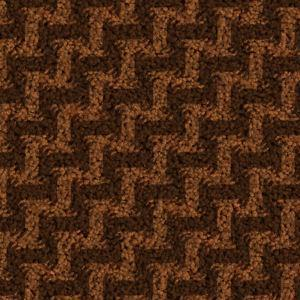
\includegraphics[width=0.13\linewidth ]{./figs/Fabric/147.jpg} & 
\hspace{-2mm} 
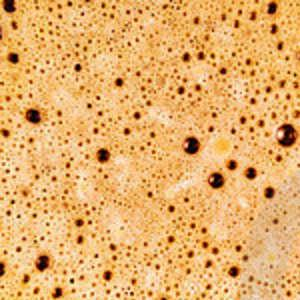
\includegraphics[width=0.13\linewidth]{./figs/fig8/bing_foam_150.jpg} & 
\hspace{-2mm}
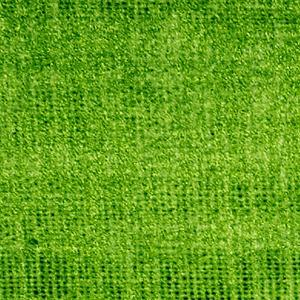
\includegraphics[width=0.13\linewidth]{./figs/Fabric/161.jpg} & 
\hspace{-2mm}
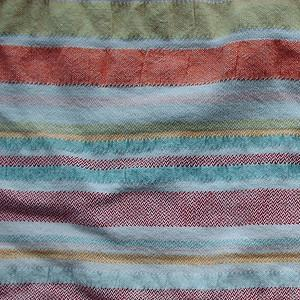
\includegraphics[width=0.13\linewidth]{./figs/Fabric/696.jpg} & 
\hspace{-2mm}
\includegraphics[width=0.13\linewidth]{./figs/Fabric/flickr_Fabric_75.jpg} \\ 

\hspace{-1.5mm}
\includegraphics[width=0.19\linewidth]{./figs/Fabric/147_syn.jpg} & 
\hspace{-3mm} 
\includegraphics[width=0.19\linewidth]{./figs/fig8/bing_foam_150_m.jpg} & 
\hspace{-3mm} 
\includegraphics[width=0.19\linewidth]{./figs/Fabric/161_syn.jpg} & 
\hspace{-3mm}
\includegraphics[width=0.19\linewidth]{./figs/Fabric/696_syn.jpg} & 
\hspace{-3mm}
\includegraphics[width=0.19\linewidth]{./figs/Fabric/flickr_Fabric_75_q.jpg} \\ 

% \scriptsize{\text{(a) 0.83, Quilting~\cite{Efros:sig2001}}} & 
% \scriptsize{\text{(b) 0.63, MMRF~\cite{paget:tip98}}} & 
% \scriptsize{\text{(c) 0.54, Phase~\cite{random:phase}}} & 
% \scriptsize{\text{(d) 0.27, Wavelets~\cite{Portilla:2000:IJCV}}} & 
% \scriptsize{\text{(e) 0.12, Quilting~\cite{Efros:sig2001}}}  \\

\hspace{-1.5mm}
\scriptsize{\text{(a) 0.83}} & 
\hspace{-3mm}
\scriptsize{\text{(b) 0.63}} & 
\hspace{-3mm}
\scriptsize{\text{(c) 0.54}} & 
\hspace{-3mm}
\scriptsize{\text{(d) 0.27}} & 
\hspace{-3mm}
\scriptsize{\text{(e) 0.12}}  \\

\hspace{-1mm}
\includegraphics[width=0.13\linewidth ]{./figs/fig8/google_brick_32.jpg} & 
\hspace{-2mm}
\includegraphics[width=0.13\linewidth]{./figs/fig8/flickr_carpet_325.jpg} & 
\hspace{-2mm}
\includegraphics[width=0.13\linewidth]{./figs/fig8/bing2_rust_136.jpg} & 
\hspace{-2mm} 
\includegraphics[width=0.13\linewidth]{./figs/fig8/bing2_pasta_69.jpg} & 
\hspace{-2mm}
\includegraphics[width=0.13\linewidth]{./figs/fig8/bing2_crowd_176.jpg} \\


% \scriptsize{\text{(f) 0.94, Quilting~\cite{Efros:sig2001}}} & 
% \scriptsize{\text{(h) 0.79, Wavelets~\cite{Portilla:2000:IJCV}}} & 
% \scriptsize{\text{(i) 0.78, MMRF~\cite{paget:tip98}}} & 
% \scriptsize{\text{(g) 0.42, MMRF~\cite{paget:tip98}}} & 
% \scriptsize{\text{(j) 0.20, Quilting~\cite{Efros:sig2001}}}  \\
\hspace{-1.5mm}
\includegraphics[width=0.19\linewidth]{./figs/fig8/google_brick_32_q.jpg} & 
\hspace{-3mm} 
\includegraphics[width=0.19\linewidth]{./figs/fig8/flickr_carpet_325_w.jpg} & 
\hspace{-3mm}
\includegraphics[width=0.19\linewidth]{./figs/fig8/bing2_rust_136_m.jpg} & 
\hspace{-3mm} 
\includegraphics[width=0.19\linewidth]{./figs/fig8/bing2_pasta_69_q.jpg} & 
\hspace{-3mm}
\includegraphics[width=0.19\linewidth]{./figs/fig8/bing2_crowd_176_q.jpg} \\ 

\hspace{-1.5mm}
\scriptsize{\text{(f) 0.74}} & 
\hspace{-3mm}
\scriptsize{\text{(g) 0.68}} & 
\hspace{-3mm}
\scriptsize{\text{(h) 0.49}} & 
\hspace{-3mm}
\scriptsize{\text{(i) 0.23}} & 
\hspace{-3mm}
\scriptsize{\text{(j) 0.19}}  \\
\end{array}$ }
\caption{Synthesizability scores of texture examples and the `best'
  synthesized textures by ETS methods. Top: exemplar; bottom:
  synthesized. }
  \label{fig:scoring1}
\end{figure*}


\begin{figure*} [!t]
  \centering \scalebox{1}{
   $ \begin{array}{cccccc}
\hspace{-1.5mm}
\includegraphics[width=0.13\linewidth ]{./figs/best/google_plastic_19.jpg} & 
\hspace{-3mm} 
\includegraphics[width=0.17\linewidth]{./figs/best/google_plastic_19_q.jpg} & 
\hspace{-3mm}
\includegraphics[width=0.17\linewidth]{./figs/best/google_plastic_19_w.jpg} & 
\hspace{-2.5mm}
\includegraphics[width=0.13\linewidth]{./figs/best/bing2_rain_163.jpg} & 
\hspace{-3mm}
\includegraphics[width=0.17\linewidth]{./figs/best/bing2_rain_163_m.jpg} & 
\hspace{-3mm}
\includegraphics[width=0.17\linewidth]{./figs/best/bing2_rain_163_q.jpg} \\ 

\hspace{-1.5mm}
\scriptsize{\text{(a) exemplar}} & 
\hspace{-3mm}
\scriptsize{\text{(b) suggested (Quilting~\cite{Efros:sig2001})}} & 
\hspace{-3mm}
\scriptsize{\text{(c) random (Wavelet~\cite{Portilla:2000:IJCV})}} & 
\hspace{-1.5mm}
\scriptsize{\text{(d) exemplar}} & 
\hspace{-3mm}
\scriptsize{\text{(e) suggested (MMRF~\cite{paget:tip98})}} & 
\hspace{-3mm}
\scriptsize{\text{(f) random (Quilting~\cite{Efros:sig2001})}}  \\

\end{array}$ }
\caption{The synthesized results of two texture examples by our suggested method and a randomly chosen method.}
  \label{fig:best}
\end{figure*}


\textbf{Qualitative evaluation}. 
Fig.~\ref{fig:synlity} and
Fig.~\ref{fig:scoring1} show examples together with their predicted
synthesizability. The synthesizability predictor here was trained
with all annotated images except for the image itself given for prediction.
% , as 
% the maximum power of the system should also be exploited. 
As can be seen, homogeneous, repetitive, and regular texture examples
obtain higher scores. The low scores are caused by many factors, such
as outliers, surface distortions, and complex structures. In
Fig.~\ref{fig:scoring1}, the `best' synthesised images by the ETS
methods are also shown.  The quality of the synthesized images is
largely consistent with the predicted synthesizability score. This is
crucial because it allows us to detect textures -- also as image
parts, see shortly -- that can be synthesized well.  As already
claimed, the system can also suggest the `best' synthesis method for a
given texture example. Fig.~\ref{fig:best} shows two such examples,
where results of the suggested method and results of a randomly chosen
method are compared.  It can be seen that our `adaptive selection' is
superior to random guessing. This is due to the fact the ETS methods
all have their own philosophies and each one works better than the
others for some textures, which necessariate an adaptive
selection for the `best' synthesis methods for a given texture example.


% , and to
% select the appropriate method to do so.

\textbf{Failure cases}. Of course, the method fails sometimes.  The
typical false positives (a high synthesizability score assigned to an
image hard to synthesize) are images with fine, global, but irregular
structures, \eg crumpled paper and fabric, wood with year rings,
foliage nerves, or hairs.  It is hard to for the features to capture
these subtle, but semantically crucial information. The typical false
negatives (low score for synthesizable images) are heterogeneous
textures such as some rust and cloud examples.  This is probably
because the space of valid textures for those is very large so that
synthesized textures more easily fall inside the space. See
Fig.~\ref{fig:failure} for such examples.

\textbf{Synthesizability with scales} Textures in an image can be
perceived and may differ at different scales. Thus, it is interesting
to see how scales of textures affects their
synthesizability. Fig.~\ref{fig:scale} shows an example, where three
scales of the same texture are used as the examples for
synthesizability prediction. Zooming in, the synthesizability score
drops -- as long as the same `textons' matter -- as those textons 
increasingly take on the role of individual objects. This is in keeping with
human intuition. 



\begin{figure} 
 \centering
\includegraphics[width=0.8\linewidth]{./figs/AP_curve_all.pdf} \\ 
\caption{The average precision of synthesizability prediction for different levels of recall, when all features are used. }
  \label{fig:curve}
\end{figure}


\begin{figure} 
  \centering
   $ \begin{array}{cccc}

\hspace{-1mm}
\includegraphics[width=0.19\linewidth]{./figs/failure/fp/bing2_crowd_35.jpg} & 
\hspace{-3mm}
%\multirow{2}{c|}{Head 1}
\includegraphics[width=0.29\linewidth, height=23mm]{./figs/failure/fp/bing2_crowd_35_m.jpg} & 
\hspace{-3mm}
\includegraphics[width=0.19\linewidth]{./figs/failure/fp/bing_hair_263.jpg} & 
\hspace{-3mm}
%\multirow{2}{c|}{Head 1}
\includegraphics[width=0.29\linewidth, height=23mm]{./figs/failure/fp/bing_hair_263_q.jpg} \\ 
\hspace{-1mm}
\scriptsize{\text{ (a) 0.65}} & 
\hspace{-3mm}
\scriptsize{\text{ (b) synthesized}  } & 
\hspace{-3mm}
\scriptsize{\text {(c) 0.59}} & 
\hspace{-3mm}
\scriptsize{\text{(d) synthesized}} \\ 

\hspace{-1mm}
\includegraphics[width=0.19\linewidth]{./figs/failure/fn/bing2_cloud_40.jpg} & 
\hspace{-3mm}
%\multirow{2}{c|}{Head 1}
\includegraphics[width=0.29\linewidth, height=23mm]{./figs/failure/fn/bing2_cloud_40_m.jpg} & 
\hspace{-3mm}
\includegraphics[width=0.19\linewidth]{./figs/failure/fn/bing2_rust_10.jpg} & 
\hspace{-3mm}
%\multirow{2}{c|}{Head 1}
\includegraphics[width=0.29\linewidth, height=23mm]{./figs/failure/fn/bing2_rust_10_m.jpg} \\ 
\hspace{-1mm}
\scriptsize{\text{ (e) 0.35}} & 
\hspace{-3mm}
\scriptsize{\text{ (f) synthesized}  } & 
\hspace{-3mm}
\scriptsize{\text {(g) 0.25}} & 
\hspace{-3mm}
\scriptsize{\text{(h) synthesized}} \\ 

\end{array}$
\caption{Failure cases: the top shows false positives and the bottom
  false negatives. Exemplars are of $300 \times 300$ pixels.}
  \label{fig:failure}
\end{figure}


\begin{figure} 
  \centering
   $ \begin{array}{ccc}
\hspace{-1.5mm}
\includegraphics[width=0.325\linewidth]{./figs/scale/flickr_crushed_78.jpg} & 
\hspace{-3mm}
\includegraphics[width=0.325\linewidth]{./figs/scale/flickr_crushed_79.jpg} & 
\hspace{-3mm}
\includegraphics[width=0.325\linewidth]{./figs/scale/flickr_crushed_80.jpg} \\
\hspace{-1.5mm}
\scriptsize{\text{ (a) 0.22}} & 
\hspace{-3mm}
\scriptsize{\text{ (b) 0.34}} & 
\hspace{-3mm}
\scriptsize{\text{ (c) 0.43}} \\ 
\end{array}$
\caption{Synthesizability for different scales of the same texture. }
  \label{fig:scale}
\end{figure}


% We also show and compare the synthesizability of different texture
% categories (the average synthesizability of all images of the
% category).  The UIUC texture dataset~\cite{UIUC:Texture}, which
% contains $25$ texture categories, each with $40$ images. Fig.~\ref{}
% shows the synthesizability of all categories (average of
% synthesizability of all texture examples in each category). From the
% figure, we find that ...

% This characterization could be further analyzed in terms of different
% texture materials, different illumination conditions, different scales
% of textures, and so on. The characterization of textures of
% Columbia-Utrecht Reflectance and Texture
% Database~\cite{columbia:texture} and Open-Surface
% dataset~\cite{open:surface} is planned as a future work. The former
% one is about different illuminations, and the latter is for real-world
% semantic textures.




\subsection{Trimming texture examples}
In this section, image synthesizability is used for trimming images to
more synthesizable parts. Given an image, the synthesizability of
subimages is computed and compared. The most synthesizable subimage is
then suggested. See Fig.~\ref{fig:roi} for examples. $500$ sub-windows
were randomly sampled, with a minimum size of $100 \times 100$ pixels
and maximum size that of the entire image.  The figure suggests that
our method performs well for this task. It is thus possible to pick
synthesizable texture examples from unconstrained images.
Fig.\ref{fig:roisyn} illustrates that synthesis is superior for the
selected windows compared to using the entire image.  Note that if two
windows receive the same/close synthesizability score, we prefer the
larger window.

%  A method to detect the synthesizable textures in images is very
% useful.
% This trimming shares some similarity with~\cite{dominant:texture:09}
% but is still different. They detect the
% dominant texture within an image; we are interested in detecting the
% most synthesizable parts.

% \subsection{Texture recognition}
% In this section, we evaluate the usefulness of synthesizability and
% the $4$ designed features (synfets) for texture recognition. The UIUC
% texture dataset~\cite{UIUC:Texture} was used for this task, which
% contains $25$ texture categories, each with $40$ images. Linear SVMs
% were used as the classifier, with $C=10$. We show the classification
% accuracy of Uniform LBP~\cite{lbp:2002}, of synfets, and of their
% concatenation. For all experiments, $12$ training images per
% class were used, and the reported accuracy was computed over $10$
% random training-test splits. The results are listed in
% Table~\ref{table:recognition}, which shows that synfets complement
% normal texture features for texture recognition. More generally, the
% self-relationships captured by our designed features also play roles
% in defining texture categories.

% {\bf I'M NOT SURE WE WANT THIS SECTION IN AT ALL. ACTUALLY, I 
% THINK WE SHOULD DROP THIS SECTION ON RECOGNITION, IRRESPECTIVE 
% OF ANY DEMANDS BY THE REVIEWERS OR AC. SYNFETS INCREASE THE 
% CLASSIFICATION SCORE WITH ABOUT 1.5%, WHILE STAYING BELOW 70%. 
% GOING UP 1.5% MAY BE OK IF LBP BRINGS YOU AROUND 98% AND WITH 
% SYNFETS ONE COMES AROUND 99.5%… BUT NOT IF BELOW 70%. A VERY 
% SMALL ADVANTAGE COMES AT THE COST OF ADDING 4 EXPENSIVE FEATURES 
% TO THE VERY SIMPLE AND SINGLE LBP… 
% THE OBVIOUS Q IS WHETHER ONE COULD NOT DO BETTER BY ADDING ANOTHER
% SIMPLE FEATURE… 
% AT THE END OF A NICE PAPER, THIS SECTION RUINS IT. THE ONLY 
% CONCLUSION ONE CAN DRAW HERE IS THAT THE SYNFETS MAY BE GOOD
% FOR SYNTHESIZABILITY, BUT ARE PRETTY USELESS FOR RECOGNITION.
% IT COULD BE THAT YOUR REFER TO RECOGNITION EARLY ON IN THE PAPER.
% WHEN DROPPING THIS SECTION, SUCH REFERENCES TO THE LATER TESTING
% OF RECOGNITION SHOULD ALSO BE ELIMINATED.}

% \subsection{Describing textures}
% We also validate the effectiveness of the four designed
% features as general texture attributes. The evaluation is based on pairwise
% comparison: given an image pair, we predict which image exhibits the
% attributes more than the other. The prediction results are compared to
% manual annotation for evaluation.  For this purpose, we labeled
% $600$ randomly chosen image pairs from the $2000$ general textures in
% terms of the comparison of the four texture
% attributes. Table~\ref{table:fet} lists the accuracy of the
% predictions.  The results show that the methods we designed for the
% four general texture attributes perform fairly well: the computed 
% comparisons correlate well with the human comparisons. We use the four
% features for synthesizability learning, but they can be used for other
% tasks as well, such as texture indexing. 



\begin{figure*} [!t]
  \centering
   $ \begin{array}{cccc}
\hspace{-1mm}
\includegraphics[width=0.24\linewidth, height=32mm]{./figs/2/2.jpg} & 
\hspace{-3mm}
\includegraphics[width=0.24\linewidth, height=32mm]{./figs/2/3.jpg} & 
\hspace{-3mm}
\includegraphics[width=0.24\linewidth, height=32mm]{./figs/2/roi_11_rect.pdf} & 
\hspace{-3mm}
\includegraphics[width=0.24\linewidth, height=32mm]{./figs/2/22_3.jpg} \\
\hspace{-1mm}
\scriptsize{\text{ (a) RS:0.50 \hspace{1mm} IS:0.19}} & 
\hspace{-3mm}
\scriptsize{\text{ (b) RS:0.40, \hspace{1mm} IS:0.22}}  &
\hspace{-3mm}
\scriptsize{\text{ (c) RS:0.53, \hspace{1mm} IS:0.40}} & 
\hspace{-3mm}
\scriptsize{\text{ (d) RS:0.51 \hspace{1mm} IS:0.23}} \\ 
\end{array}$
\caption{The most synthesizable region as detected. The synthesizability
  of the whole images (IS) vs. the selected region (RS) are given.}
  \label{fig:roi}
\end{figure*}


\begin{figure} 
  \centering
   $ \begin{array}{ccc}
\hspace{-1.5mm}
\includegraphics[width=0.30\linewidth]{./figs/roi/roi_2.jpg} & 
\hspace{-3mm}
\includegraphics[width=0.33\linewidth, height=21mm]{./figs/roi/2_syn.jpg} & 
\hspace{-3mm}
\includegraphics[width=0.33\linewidth, height=21mm]{./figs/roi/2_1_syn.jpg} \\

\hspace{-1.5mm}
\scriptsize{ \text{(a) IS:0.14 \hspace{1mm} RS:0.43}} & 
\hspace{-3mm}
\scriptsize{\text{(b) Synthesized from image}} & 
\hspace{-3mm}
\scriptsize{\text{(c) Synthesized from region}} \\
 
\hspace{-1.5mm}
\includegraphics[width=0.30\linewidth]{./figs/roi/roi_1.jpg} & 
\hspace{-3mm}
\includegraphics[width=0.33\linewidth, height=21mm]{./figs/roi/1_syn.jpg} & 
\hspace{-3mm}
\includegraphics[width=0.33\linewidth, height=21mm]{./figs/roi/1_1_syn.jpg} \\
\hspace{-1.5mm}
\scriptsize{\text{(d) IS:0.13 \hspace{1mm} RS:0.50}} & 
\hspace{-3mm}
\scriptsize{\text{(e) Synthesized from image}} & 
\hspace{-3mm}
\scriptsize{\text{(f) Synthesized from region}} \\ 

\end{array}$
\caption{Synthesis results for the images on the left, starting from 
  the entire image (IS; mid column) vs. from the selected region (RS;
  right column).}
  \label{fig:roisyn}
\end{figure}

% \begin{table}[tb] \footnotesize 
% $\begin{array}{ccccc}
% \begin{tabular}{c|}
% \multicolumn{1}{c|}{Feature} \\ \hline 
% Accuracy (\%) \\ 
% \end{tabular}

% \begin{tabular}{c}
% \multicolumn{1}{c}{\scriptsize{LBP}} \\ \hline 
% 68.1 (2.1)  \\ 
% \end{tabular}

% \begin{tabular}{c}
% \multicolumn{1}{c}{\scriptsize{Synfets}} \\ \hline
% 31.1 (1.6)   \\ 
% \end{tabular}

% \begin{tabular}{c}
% \multicolumn{1}{c}{\scriptsize{LBP + Synfets}} \\ \hline 
% 69.7(1.6)   \\ 
% \end{tabular}
% \end{array} $
% \vspace{1mm}
% \centering 
% \caption{Classification accuracy on Texture-25 dataset.} \label{table:recognition}
% \end{table}




% \begin{table} \footnotesize 
% $\begin{array}{ccccc}
% \begin{tabular}{c|c}
% \multicolumn{1}{c|}{Features} \\ \hline
% Accuracy \\  
% \end{tabular}

% \begin{tabular}{c}
% \multicolumn{1}{c}{\scriptsize{Textureness}} \\ \hline 
% 89.1\%  \\
% \end{tabular}

% \begin{tabular}{c}
% \multicolumn{1}{c}{\scriptsize{Homogeneity}} \\ \hline 
% 79.4\%  \\ 
% \end{tabular}

% \begin{tabular}{c}
% \multicolumn{1}{c}{\scriptsize{Repetitiveness}} \\ \hline 
% 82.5\%  \\ 
% \end{tabular}

% \begin{tabular}{c}
% \multicolumn{1}{c}{\scriptsize{Regularity}} \\ \hline 
% 75.2\%  \\ 
% \end{tabular}
% \end{array} $
% \vspace{1mm}
% \centering 
% \caption{Accuracy of the four designed texture features. 
% } \label{table:fet}
% \end{table}


\section{Conclusions}
\label{sec:conclusion}
The paper proposed synthesizability as a novel texture property and
developed a computational predictor for it. We constructed a fairly
large texture dataset and calibrated it according to
synthesizability. A set of texture features have been proposed and, in
some cases, designed for the learning, such as `textureness',
homogeneity, repetitiveness, irregularity. Extensive experiments show
that image synthesizability can be learned and predicted
computationally. It can be used to find good texture examples for
synthesis, to detect good textures from unconstrained images for
synthesis, and to choose an appropriate method to do so.

Our approach can be seen as kind of a `winner-uses-all' strategy. 
Rather than aiming for the next best method, the idea is to rather 
pick one case-optimal method among several existing alternatives,
with the goal of reaching success rates better than those of any 
individual method. Such eclectic strategy could also be tried for 
other tasks: rather than creating ever stronger methods, choose 
from existing methods based on some preprocessing. 

\noindent
\textbf{Reproducibility.} The Code, Data and more examples are
available at: \url{www.vision.ee.ethz.ch/~daid/synthesizability}.

\vspace{1mm}
\noindent
\textbf{Acknowledgement.} The work is supported by the ERC Advanced Grant VarCity and 
the ETH-Singapore project Future Cities.

{\footnotesize
\bibliographystyle{ieee}
\bibliography{egbib}
}

\end{document}
